% Made up for the tikra benchmark.
\usepgfplotslibrary{statistics}
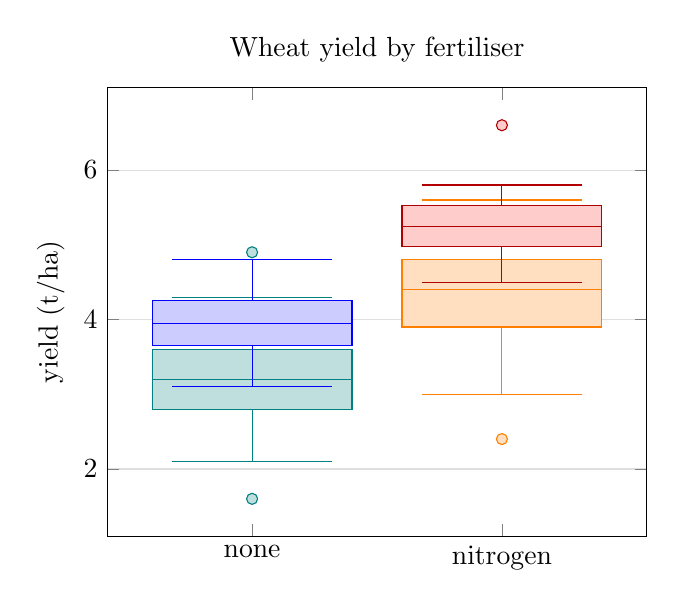
\begin{tikzpicture}
\begin{axis}[boxplot/draw direction=y, ylabel={yield (t/ha)}, title={Wheat yield by fertiliser},
    xtick={1,2,3,4}, xticklabels={none, nitrogen, compost, both}, ymajorgrids,
    grid style={gray!25}, cycle list={{teal,fill=teal!25},{orange,fill=orange!25},{blue,fill=blue!20},{red!70!black,fill=red!20}}]
  \addplot+[boxplot prepared={lower whisker=2.1, lower quartile=2.8, median=3.2,
      upper quartile=3.6, upper whisker=4.3}] coordinates {(0,1.6) (0,4.9)};
  \addplot+[boxplot prepared={lower whisker=3.0, lower quartile=3.9, median=4.4,
      upper quartile=4.8, upper whisker=5.6}] coordinates {(0,2.4)};
  \addplot+[boxplot] table[row sep=\\, y index=0] {
    3.1\\ 3.8\\ 4.0\\ 4.2\\ 3.5\\ 4.6\\ 3.9\\ 4.1\\ 3.3\\ 4.4\\ 4.8\\ 3.7\\ };
  \addplot+[boxplot] table[row sep=\\, y index=0] {
    4.5\\ 5.2\\ 5.0\\ 5.6\\ 4.9\\ 5.8\\ 5.3\\ 4.7\\ 5.5\\ 6.6\\ 5.1\\ 5.4\\ };
\end{axis}
\end{tikzpicture}
